\ifdefined\beamerclass
\else
    \def\beamerclass{beamer}
\fi
\documentclass[\beamerclass]{beamer}

\usepackage{pgfpages}
\mode<handout>{
  % \setbeamercolor{background canvas}{bg=black!20}
  \pgfpagesuselayout{2 on 1}[a4paper,border shrink=5mm]
}

\usepackage[english]{babel}
\usepackage{algorithm}
\usepackage[noend]{algpseudocode}
\usepackage[utf8x]{inputenc}
\usepackage{graphicx}
\usepackage{hyperref}
%\graphicspath{{./images/}}
\usepackage{tikz}
\usetikzlibrary{shapes.geometric, arrows,chains}
\usepackage{booktabs,makecell,multirow,tabularx}
\usepackage{verbatim}
\renewcommand{\arraystretch}{1.2}
\renewcommand\theadfont{\normalfont\bfseries}
\usepackage{array}
\usepackage{listings}
\lstset{language=Java, showstringspaces=false}
\usepackage[normalem]{ulem}
\usepackage{bm}
\def\layersep{2.5cm}

\usepackage{xcolor}
%\usepackage{subfig}
\setbeamertemplate{caption}{\insertcaption}
\usepackage[caption=false]{subfig}
\usepackage{hyperref}
\usepackage{verbatim}
%\setbeamertemplate{caption}[numbered]%\numberwithin{figure}{section}
% Define block styles
\tikzstyle{decision} = [diamond, draw, fill=blue!20, 
    text width=4.5em, text badly centered, node distance=3cm, inner sep=0pt]
\tikzstyle{block} = [rectangle, draw, fill=blue!20, 
    text width=3em, text centered, rounded corners, minimum height=3em]
\tikzstyle{line} = [draw, -latex']
\tikzstyle{cloud} = [draw, ellipse, fill=red!20, node distance=3cm,
    minimum height=2em]
\tikzset{
  startstop/.style={
    rectangle, 
    rounded corners,
    minimum width=3cm, 
    minimum height=1cm,
    align=center, 
    draw=black, 
    fill=red!30
    },
  process/.style={
    rectangle, 
    minimum width=3cm, 
    minimum height=1cm, 
    align=center, 
    draw=black, 
    fill=blue!30
    },
  decision/.style={
    rectangle, 
    minimum width=3cm, 
    minimum height=1cm, align=center, 
    draw=black, 
    fill=green!30
    },
  arrow/.style={thick,->,>=stealth},
  dec/.style={
    ellipse, 
    align=center, 
    draw=black, 
    fill=green!30
    },
}
\tikzstyle{arrow} = [thick,->,>=stealth]

\tikzset{onslide/.code args={<#1>#2}{%
  \only<#1>{\pgfkeysalso{#2}} % \pgfkeysalso doesn't change the path
}}

\makeatletter
\newenvironment<>{btHighlight}[1][]
{\begin{onlyenv}#2\begingroup\tikzset{bt@Highlight@par/.style={#1}}\begin{lrbox}{\@tempboxa}}
{\end{lrbox}\bt@HL@box[bt@Highlight@par]{\@tempboxa}\endgroup\end{onlyenv}}

\newcommand<>\btHL[1][]{%
  \only#2{\begin{btHighlight}[#1]\bgroup\aftergroup\bt@HL@endenv}%
}
\def\bt@HL@endenv{%
  \end{btHighlight}%   
  \egroup
}
\newcommand{\bt@HL@box}[2][]{%
  \tikz[#1]{%
    \pgfpathrectangle{\pgfpoint{1pt}{0pt}}{\pgfpoint{\wd #2}{\ht #2}}%
    \pgfusepath{use as bounding box}%
    \node[anchor=base west, fill=orange!30,outer sep=0pt,inner xsep=1pt, inner ysep=0pt, rounded corners=3pt, minimum height=\ht\strutbox+1pt,#1]{\raisebox{1pt}{\strut}\strut\usebox{#2}};
  }%
}
\makeatother




\usetheme{Copenhagen}
\hypersetup{pdfstartview={Fit}}
\lstset{basicstyle=\small\ttfamily,breaklines=true}

\title[COMP6248 Deep Learning]{Review of Machine Learning}
\subtitle{(and some Deep Learning)}
\author{Jonathon Hare}
\institute[]
{
  Vision, Learning and Control\\
  University of Southampton 
}
\date{}
\subject{Computer Science}
\useoutertheme{infolines}
\setbeamertemplate{headline}{} %remove headline
\setbeamertemplate{navigation symbols}{} %remove navigation symbols

\begin{document}
\begin{frame}
  \titlepage
\end{frame}
%%-------------------------------------------------------------%

\begin{frame}[fragile]\frametitle{Types of Learning}
\begin{itemize}
\item Supervised Learning - learn to predict an output when given an input vector

\item Unsupervised Learning - discover a good internal representation of the input

\item Reinforcement Learning - learn to select an action to maximize the expectation of future rewards (payoff)

\item Self-supervised Learning - learn with targets induced by a prior on the unlabelled training data

\item Semi-supervised Learning - learn with few labelled examples and many unlabelled ones
\end{itemize}

\end{frame}
%%-------------------------------------------------------------%

\begin{frame}[fragile]\frametitle{Supervised Learning}
\center{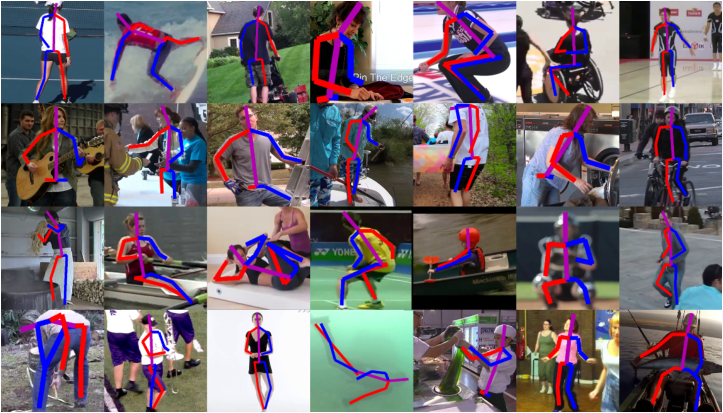
\includegraphics[width=.9\textwidth]{figs/SL.pdf}} \\
\footnotesize{Newell, Alejandro, Kaiyu Yang, and Jia Deng. ``Stacked hourglass networks for human pose estimation.'' ECCV'16. Springer, 2016.}
\end{frame}
%%-------------------------------------------------------------%

\begin{frame}[fragile]\frametitle{Unsupervised Learning}
\center{\includegraphics[width=7cm]{figs/UL.pdf}}
\footnotesize{\url{https://skymind.ai/wiki/generative-adversarial-network-gan} and \url{https://github.com/robbiebarrat/art-DCGAN}}
\end{frame}
%%-------------------------------------------------------------%

\begin{frame}[fragile]\frametitle{Reinforcement Learning}
\center{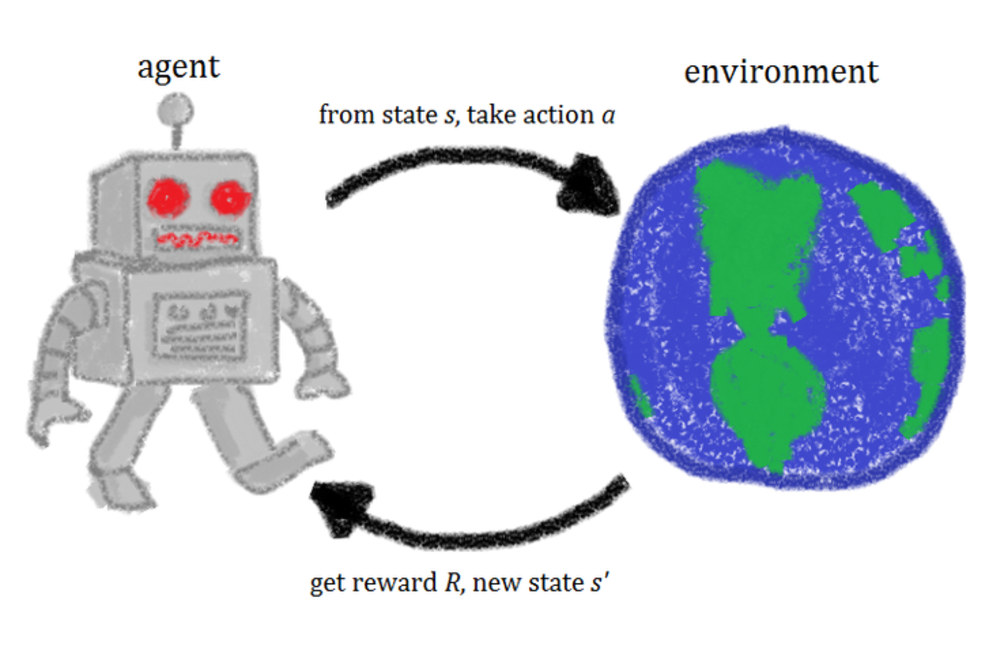
\includegraphics[width=\textwidth]{figs/RL.pdf}}
\footnotesize{Reference: Wikipedia \url{https://simple.wikipedia.org/wiki/Reinforcement_learning}}
\end{frame}
%%-------------------------------------------------------------%

\begin{frame}[fragile]\frametitle{Self-supervised Learning}
% \center{\includegraphics[width=7cm]{figs/UL.pdf}}
% \footnotesize{\url{https://skymind.ai/wiki/generative-adversarial-network-gan} and \url{https://github.com/robbiebarrat/art-DCGAN}}
\end{frame}
%%-------------------------------------------------------------%

\begin{frame}[fragile]\frametitle{Semi-supervised Learning}
% \center{\includegraphics[width=7cm]{figs/UL.pdf}}
% \footnotesize{\url{https://skymind.ai/wiki/generative-adversarial-network-gan} and \url{https://github.com/robbiebarrat/art-DCGAN}}
\end{frame}
%%-------------------------------------------------------------%


\begin{frame}[fragile]\frametitle{Two Types of Supervised Learning}
\begin{itemize}
\item Classification:  The program is asked to specify which of $k$ categories some input belongs to. The learning algorithm produces a function $f : \mathbb{R}^n \rightarrow \{1, ..., k\}$.

\item Regression:  The program is asked predict a numerical value given some input. The learning algorithm outputs a function $f: \mathbb{R}^n \rightarrow \mathbb{R}$.
\end{itemize}
\end{frame}
%%-------------------------------------------------------------%


\begin{frame}[fragile]\frametitle{How Supervised Learning Typically Works}
\begin{itemize}
\item Start by choosing a model-class: $\hat y = f(\bm x; \bm W)$ where the model-class $f$ is a way of using some numerical parameters, $\bm W$, to map each input vector $\bm x$ to a predicted output $ \hat y$.
\item Learning means adjusting the parameters to reduce the discrepancy between the target output $ y$ on each training case and the output $\hat y$, predicted by the model. %\footnote{Reference: Geoffrey Hinton \url{https://www.cs.toronto.edu/~hinton/coursera/lecture1/lec1e.mp4}}
\end{itemize}

\end{frame}
%%-------------------------------------------------------------%

\begin{frame}[fragile]\frametitle{Generative vs. Discriminative Models}
Generative vs. discriminative approaches to classification use different statistical modelling.
\begin{itemize}
\item Generative models model the distribution of individual classes. Given an observable variable $X$ and a target variable $Y$, a generative model is a statistical model that tries to model $P[X|Y]$ and $P[Y]$ in order to model the joint probability distribution $P[X, Y]$. 
\item Discriminative models learn the boundary between classes.  A discriminative models is a model of the conditional probability of the target $Y$, given an observation $X$, $P[Y|X; W]$.  \footnote{Reference: \url{https://en.wikipedia.org/wiki/Generative_model}}
\end{itemize} 

Additional Reading
\url{http://cs229.stanford.edu/notes/cs229-notes2.pdf}
%\url{http://robotics.stanford.edu/~ang/papers/nips01-discriminativegenerative.pdf}
\end{frame}
%%-------------------------------------------------------------%

%\begin{frame}[fragile]\frametitle{Deep Generative Models}
%
%Deep Generative Models (DGMs) are generative models that use ideas from deep learning.
%\begin{itemize}
%\item Autoencoder (AE) based models have an encoder and decoder. Popular models in this category are Variational autoencoders (VAEs), Deep Recurrent Attentive Writer (DRAW), Denoising VAEs, and Wasserstein AEs. 
%\item Autoregressive models include PixelCNN, PixelRNN, Wavenet.
%\end{itemize}
%\footnote{Recent Trends in Deep Generative Models: a Review \url{https://ieeexplore.ieee.org/stamp/stamp.jsp?tp=&arnumber=8566353}}
%\end{frame}
%%%%-------------------------------------------------------------%


\begin{frame}[fragile]\frametitle{Multilayer Perceptron}
\begin{tikzpicture}[shorten >=1pt,->,draw=black!50, node distance=\layersep]
    \tikzstyle{every pin edge}=[<-,shorten <=1pt]
    \tikzstyle{neuron}=[circle,fill=black!25,minimum size=17pt,inner sep=0pt]
    \tikzstyle{input neuron}=[neuron, fill=green!50];
    \tikzstyle{output neuron}=[neuron, fill=red!50];
    \tikzstyle{hidden neuron}=[neuron, fill=blue!50];
    \tikzstyle{annot} = [text width=4em, text centered]

    % Draw the input layer nodes
    \foreach \name / \y in {1,...,4}
    % This is the same as writing \foreach \name / \y in {1/1,2/2,3/3,4/4}
        \node[input neuron] (I-\name) at (0,-\y) {$x_\y$};

    % Draw the hidden layer nodes
    \foreach \name / \y in {1,...,5}
        \path[yshift=0.5cm]
            node[hidden neuron] (H-\name) at (1.5*\layersep,-\y cm) {$h_\y$};

    % Draw the output layer node
        \foreach \name / \y in {1,...,2}
        \path[yshift=0.5cm]
            node[output neuron, pin={[pin edge={->}]right:$\hat y_\y$}, right of=H-3] (O-\name) at (1.5*\layersep,-40-\y cm) {$o_\y$};
    %\node[output neuron,pin={[pin edge={->}]right:Output}, right of=H-3] (O) {o};

    % Connect every node in the input layer with every node in the
    % hidden layer.
    \path (I-1) edge node[anchor=south] {$w_{ji}^{(1)}$}(H-1);
   \foreach \source in {1,...,4}
        \foreach \dest in {1,...,5}
       % \draw [arrow] (I-\source) - (H-\dest);
            \path (I-\source) edge (H-\dest) ;

    % Connect every node in the hidden layer with the output layer
    \path (H-1) edge node[anchor=south] {$w_{kj}^{(2)}$}(O-1);
    \foreach \source in {1,...,5}
       \foreach \dest in {1,...,2}
        \path (H-\source) edge (O-\dest);

    % Annotate the layers
    \node[annot,above of=H-1, node distance=1cm] (hl) {Hidden layer};
    \node[annot,left of=hl] {Input layer};
    \node[annot,right of=hl] {Output layer};
\end{tikzpicture}
\end{frame}

%-------------------------------------------------------------%

\begin{frame}[fragile]\frametitle{Review: Batch Gradient Descent}

\bf{begin initialize} $n_H$, $w$, $Th$, $\eta$, $m \leftarrow 0$,  $r \leftarrow 0$ \\
\hspace{1cm} \bf{do } $r \leftarrow r + 1$ (increment epoch) \\
\hspace{2cm} $m \leftarrow 0$; $\Delta w \leftarrow 0$ \\
\hspace{2cm} do $m \leftarrow m + 1$ \\
\hspace{3cm} $x^m \leftarrow $ selected pattern \\ 
\hspace{3cm} $\Delta w \leftarrow \Delta w -  \eta \frac{\partial J}{ \partial w}$ \\
\hspace{2cm} until $m=M$ \\
\hspace{2cm} $w \leftarrow w + \Delta w$ \\
\hspace{1cm} until $J(w) < Th$ \\
return $w$ \\
end

\end{frame}
%-------------------------------------------------------------%


\begin{frame}[fragile]\frametitle{Review: Stochastic Gradient Descent}

\bf{begin initialize} $n_H$, $w$, $Th$, $\eta$, $m = 0$,  $r = 0$ \\
\hspace{1cm} \bf{do } $r \leftarrow r + 1$ (increment epoch) \\
\hspace{2cm} $m \leftarrow 0$\\
\hspace{2cm} \bf{do } $m \leftarrow m + 1$ \\
\hspace{3cm} $x^m \leftarrow$ selected pattern (randomly) \\
\hspace{3cm} $w \leftarrow w -  \eta \frac{\partial J}{ \partial w}$ \\
\hspace{2cm} until $m=M$ \\
\hspace{1cm} until $J(w) < Th$ \\
return $w$ \\
end

\end{frame}
%-------------------------------------------------------------%


\begin{frame}[fragile]\frametitle{The Cost Function (measure of discrepancy) }

Recall from Foundations of Machine Learning:
\begin{itemize}

\item Mean Squared Error (MSE) for $M$ data points is given by \\

$MSE = \frac{1}{2*M} \sum_{i=1}^M (\hat{y}_i - y_i)^2 $

\item  $\frac{1}{2*M} $ just a constant so can be replaced by $\frac{1}{2} $ or $\frac{1}{M}$
\item Other cost functions can be used as well, for example the KL divergence or Hellinger distance \footnote{https://stats.stackexchange.com/questions/154879/a-list-of-cost-functions-used-in-neural-networks-alongside-applications}

\item MSE can be slow to learn, especially if the predictions are very far off the targets \footnote{ http://neuralnetworksanddeeplearning.com/chap3.html}

\item Cross-Entropy Cost function is generally a better choice of cost function (discussed next)
\end{itemize} 

\end{frame}
%%-------------------------------------------------------------%

\begin{frame}[fragile]\frametitle{Cross-Entropy Cost Function}

\begin{itemize}
\item $J = -\frac{1}{M} \sum_x [y In(\hat y) + (1 - y) In (1 - \hat y)] $ \\ where $M$ is the number of data points in the training set
\item The cross-entropy cost function is non-negative, $J > 0$
\item $J \approx 0 $ when the prediction and targets are equal (i.e. $y = 0$ and $\hat y = 0$ or when $y = 1$ and $\hat y = 1$)
\item $\frac{\partial J}{\partial w_{ij}} $ is proportional to the error in the output ($\hat y - y$) and therefore, the larger the error, the faster the neuron will learn! %\footnote{Discuss element of surprise and information theory https://datascience.stackexchange.com/questions/9302/the-cross-entropy-error-function-in-neural-networks, good expln here: \url{https://www.youtube.com/watch?v=k_S5fnKjO-4&list=PLkDaE6sCZn6Ec-XTbcX1uRg2_u4xOEky0&index=24}}
\end{itemize}

\end{frame}
%%-------------------------------------------------------------%

\begin{frame}[fragile]\frametitle{Cross-Entropy Cost Function - What Does it Mean?}
\begin{itemize}
\item The cross-entropy can be thought of as a {\bf measure of surprise}. \\

\item Given some input $x_i$, we can think of $\hat y_i$ as the estimated probability that $x_i$ belongs to class $1$, and $1-\hat y_i$ is the estimated probability that it belongs to class $0$.

\item Note the extreme case of infinite cross-entropy, if your model believes that a class has 0 probability of occurrence, and yet the class appears in the data, the "surprise" of your model will be infinitely great. 
\end{itemize}
\end{frame}
%%-------------------------------------------------------------%

\begin{frame}[fragile]\frametitle{General Cross-Entropy Cost Function for Neural Networks}


 $J = -\frac{1}{M} \sum_{i = 1}^M \sum_{k = 1}^K [y_k^{(i)} In (\hat y_k^{(i)}) + (1 - y_k^{(i)}) In (1 - \hat y_k^{(i)})] $ \\  

where $M$ is the number of data points in the training set and $K$ is the number of classes of the classification problem, $\hat y \in \mathbb{R}^K$

%Use this reference: \url{https://www.youtube.com/watch?v=0twSSFZN9Mc}
\end{frame}
%%-------------------------------------------------------------%

\begin{frame}[fragile]\frametitle{Softmax}
The softmax is an activation function used at the output layer of a neural network that forces the outputs  to sum to 1 so that they can represent a probability distribution across a discrete mutually exclusive alternatives.

$ y_j = \frac{e^{z_j}}{\sum_{k=1}^K e^{z_j}} $, for $j = 1, 2, ..., K$

Note $\frac{\partial y_i }{z_i} = y_i (1 - y_i) $

\begin{itemize}
\item The output of a sofmax layer is a set of positive numbers which sum up to $1$ and can be thought of as a probability distribution
\end{itemize}

\end{frame}
%%-------------------------------------------------------------%

\begin{frame}[fragile]\frametitle{Softmax}
Exercise: Construct an example showing explicitly that in a network with a sigmoid output layer, the output activations won't always sum to 1.
\end{frame}
%%-------------------------------------------------------------%

\begin{frame}[fragile]\frametitle{A Quick Introduction to Tensors}
A tensor, $T$, is a generalization of vectors and matrices, which can be thought of as a multidimensional array.

\begin{itemize}
\item A $0D$ tensor is a scalar
\item A $1D$ tensor is a vector
\item A $2D$ tensor is a matrix
\item A $3D$ tensor can be thought of as a vector of identically sized matrices
\item A $4D$ tensor can be thought of as a matrix of identically sized matrices or a sequence of $3D$ tensors
\item etc.
\end{itemize}
\end{frame}
%%-------------------------------------------------------------%

\begin{frame}[fragile]\frametitle{A Quick Introduction to Tensors}
\begin{itemize}
\item A tensor is a container which can house data in $N$ dimensions. Often and erroneously used interchangeably with the matrix (which is specifically a 2-dimensional tensor), tensors are generalizations of matrices to N-dimensional space.  
\item Tensors are used to encode the data as well as the model parameters
\item Data manipulation via tensors enables CPUs and GPUs to run at peak performance
\end{itemize}
\end{frame}
%%-------------------------------------------------------------%

\begin{frame}[fragile]\frametitle{A Quick Introduction to Tensors}
Link to PyTorch Tensor Basics
\url{https://gist.github.com/kfarrahi/f8f51824b23252c81d5aaec461365e73}
\end{frame}
%-------------------------------------------------------------%
\end{document}
